\documentclass[border=5mm]{standalone}
\usepackage{tikz}
\usetikzlibrary{cd}
\usetikzlibrary{decorations.pathmorphing,shapes,shapes.misc}
\begin{document}
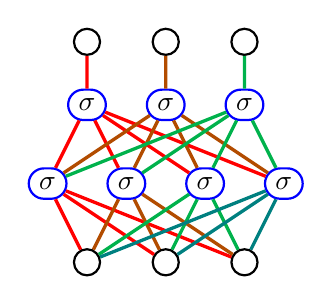
\begin{tikzpicture}
\begin{scope}[every node/.style={circle,thick,draw}]
    \node (A1) at (0.5,0) {};
    \node (A2) at (1.5,0) {};
    \node (A3) at (2.5,0) {};
    \node (D1) at (0.5,2.8) {};
    \node (D2) at (1.5,2.8) {};
    \node (D3) at (2.5,2.8) {};
\end{scope}
\begin{scope}[every node/.style={rounded rectangle,thick,draw=blue}]
    \node (B1) at (0,1) {$\sigma$};
    \node (B2) at (1,1) {$\sigma$};
    \node (B3) at (2,1) {$\sigma$};
    \node (B4) at (3,1) {$\sigma$};
    \node (C1) at (0.5,2) {$\sigma$};
    \node (C2) at (1.5,2) {$\sigma$};
    \node (C3) at (2.5,2) {$\sigma$};
\end{scope}
\begin{scope}[>={Stealth[black]},
              every edge/.style={draw=red,very thick}]
    \path [-] (A1) edge node {}(B1);
    \path [-] (A2) edge node {}(B1);
    \path [-] (A3) edge node {}(B1);
    \path [-] (B1) edge node {}(C1);
    \path [-] (B2) edge node {}(C1);
    \path [-] (B3) edge node {}(C1);
    \path [-] (B4) edge node {}(C1);
    \path [-] (C1) edge node {}(D1);
\end{scope}
\begin{scope}[>={Stealth[black]},
              every edge/.style={draw=red!70!green,very thick}]
    \path [-] (A1) edge node {}(B2);
    \path [-] (A2) edge node {}(B2);
    \path [-] (A3) edge node {}(B2);
    \path [-] (B1) edge node {}(C2);
    \path [-] (B2) edge node {}(C2);
    \path [-] (B3) edge node {}(C2);
    \path [-] (B4) edge node {}(C2);
    \path [-] (C2) edge node {}(D2);
\end{scope}
\begin{scope}[>={Stealth[black]},
              every edge/.style={draw=green!70!blue,very thick}]
    \path [-] (A1) edge node {}(B3);
    \path [-] (A2) edge node {}(B3);
    \path [-] (A3) edge node {}(B3);
    \path [-] (B1) edge node {}(C3);
    \path [-] (B2) edge node {}(C3);
    \path [-] (B3) edge node {}(C3);
    \path [-] (B4) edge node {}(C3);
    \path [-] (C3) edge node {}(D3);
\end{scope}
\begin{scope}[>={Stealth[black]},
              every edge/.style={draw=green!50!blue,very thick}]
    \path [-] (A1) edge node {}(B4);
    \path [-] (A2) edge node {}(B4);
    \path [-] (A3) edge node {}(B4);
\end{scope}
\end{tikzpicture}
\end{document}  

%
%
%
%
%
%
%
%
%
%
%
%
%
%
%
%
%
%
%
%
%
%
%
%
%
%
%
%
















